% \chapter{Feature extraction}
\chapter{特征提取}
\label{chap:feature_extraction}

% A robot can obtain information about its environment by both active (e.g., ultra-sound, light, and laser) or passive sensing (e.g., acceleration, magnetic field, or cameras). There are only few cases where this information is directly useful to a robot. Before being able to arrive at semantic information such as ``I'm in the kitchen'', ``this is a cup'' or ``this is a horse'', is identifying higher-level \emph{features}.\index{Features} 

% The goal of this chapter is to introduce a series of standard feature detectors such as the 

机器人可以通过有源(例如,超声,光和激光)或被动感测(例如,加速度,磁场或照相机)获得关于其环境的信息。只有少数情况下,这些信息对机器人直接有用。在能够得到诸如“我在厨房”之类的语义信息之前,“这是一个杯子”或者“这是一匹马”,正在识别更高层次的\emph{features}。\index{特征}

本章的目标是引入一系列标准特征检测器,如


\begin{itemize}
% \item Hough-transform to detect lines, circles and other shapes,
% \item numerical methods such as least-squares, split-and-merge and RANSAC to find high-level features in noisy data,
% \item Scale-invariant features.

\item 霍夫变换以检测线,圆和其他形状,
\item 数值方法,如最小二乘法,分割合并和RANSAC,以在嘈杂数据中查找高级功能,
\item 缩放不变特征。
\end{itemize}

% \section{Feature detection as an information-reduction problem}
% The information generated by sensors can be quite formidable. For example, a simple webcam generates 640x480 color pixels (red, green and blue) or 921600 Bytes around 30 times per second. A single-ray laser scanner still provides around 600 distance measurements 10 times per second. This is in contrast to the information that a robot actually requires. Consider for example the maze-solving competition ``Ratslife'' (Section \ref{sec:ratslife}) in which the robot's camera can be used to recognize one of 48 different color patterns (Figure \ref{fig:ratslife}) that are distributed in the environment, or the presence or absence of a charger, essentially reducing hundreds of bytes of camera data to around 6 bit ($2^6=64$ different values) content. The goal of most image processing algorithms is therefore to first reduce information content in a meaningful way and then extract relevant information. In chapter \ref{chap:vision}, we have seen convolution-based filters such as blurring, detecting edges, or binary operations such as thresholding. We are now interested in methods to extract higher-level features such as lines and techniques to extract them.

\section{功能检测作为信息减少问题}
传感器产生的信息非常强大。例如,简单的网络摄像头每秒生成640x480个彩色像素(红色,绿色和蓝色)或921600字节大约30次。单射线激光扫描仪每秒可提供约600次测距,每次10次。这与机器人实际需要的信息相反。例如,考虑例如迷宫解决竞争“Ratslife”(部分\ref{sec:ratslife}),其中机器人的相机可用于识别48种不同颜色模式之一(图\ref{fig:ratlife}),分布在环境中,或充电器的存在或不存在,基本上将数百字节的摄像机数据减少到大约6位($2^6=64$不同值)的内容。因此,大多数图像处理算法的目标是首先以有意义的方式减少信息内容,然后提取相关信息。在\ref{chap:vision}中,我们已经看到了基于卷积的过滤器,例如模糊,检测边缘或二进制操作,如阈值。我们现在对提取更高级别功能(如线条和技术)以提取它们的方法感兴趣。


% \section{Features}
\section{特征}

% Lines are particularly useful features for localization and can correspond to walls in laser scans, markers on the floor or corners detected in a camera image. Whereas a Sobel filter (Section \ref{sec:sobel}) can help us to highlight lines and edges in images, additional algorithms are needed to extract structured information such as the orientation and position of a line with respect to the robot.

% A desirable property of a feature is that its extraction is repeatable and robust to rotation, scale, and noise in the data. We need feature detectors that can extract the same feature from sensor data, even if the robot has slightly turned or moved farther or closer to the feature. There are many feature detectors available that accomplish this, prominent examples are the Harris corner detector\index{Harris Corner Detector} (essentially detecting points in the image where vertical and horizontal lines cross) and the SIFT feature detector\index{SIFT features}. Feature detection is important far beyond robotics and is for example used in hand-held cameras that can automatically stitch images together. Here, feature detectors will ``fire'' on the same features in two images taken from slightly different perspectives, which allows the camera to calculate the transformation between the two. 

% This chapter focuses on two important classes of features: line features and scale-invariant features in images (SIFT). Both features provide tangible example for the least-squares and RANSAC algorithms, which are also introduced in this chapter. Both features are representative for a large class of detectors, and have been chosen for their simplicity, providing a basis for understanding the function of more complex feature detectors. 


线是特别有用的定位特征,可以对应于激光扫描中的墙壁,地面上的标记或摄像机图像中检测到的角落。而Sobel过滤器(部分\ref{sec:sobel})可以帮助我们突出显示图像中的线条和边缘,需要额外的算法来提取结构化信息,例如相对于机器人的线的方向和位置。

特征的期望性质是其提取对于数据中的旋转,缩放和噪声是可重复的和鲁棒的。我们需要能够从传感器数据中提取相同特征的特征检测器,即使机器人稍微转动或移动得更远或更接近特征。有许多功能检测器可以实现这一点,突出的例子是Harris角检测器\index{Harris Corner Detector}(基本上是检测垂直和水平线交叉的图像中的点)和SIFT特征检测器\index{SIFT特征}。特征检测是非常重要的机器人技术,例如用在可以自动将图像拼接在一起的手持相机中。在这里,特征检测器将在从稍微不同的角度拍摄的两个图像中的相同特征上“触发”,这允许相机计算两者之间的转换。

本章重点介绍两个重要的特征:图像中的线特征和尺度不变特征(SIFT)。这两个特征为最小二乘法和RANSAC算法提供了实际的例子,本章也将介绍这一点。这两个特征都代表了一大类检测器,并且被选择为简单,为理解更复杂的特征检测器的功能提供了基础。


% \section{Line recognition}
\section{线条识别}

% Why are lines a useful feature? As you will see next chapter, the key challenge in estimating a robot's pose is unreliable odometry, in particular when it comes to turning. Here, a simple infrared sensor measuring the distance to a wall can provide the robot with a much better feel for what actually happened. Similarly, if a robot has the ability to track markers in the environment using vision, it gets another estimate on how much it is actually moving. How information from odometry and other sensors can be fused not only to localize the robot, but also to create maps of its environment, will be the focus of the remainder of this book.

% A laser scanner or similar device pointed against a wall will return a suite of $N$ points at position $(x_i,y_i)$ in the robot's coordinate system. These points can also be represented in polar coordinates $ (\rho_i,\theta_i)$. We can now imagine a line running through these points that is parametrized with a distance $r$ and an angle $\alpha$. Here, $r$ is the distance of the robot to the wall and $ \alpha$ its angle. As all sensors are noisy, each point will have distance $d_i$ from the ``optimal'' line running through the points. These relationships are illustrated in Figure \ref{fig:linefitting}.

为什么线是有用的功能?正如您将看到下一章,估计机器人姿势的关键挑战是不可靠的测距,特别是在转弯时。这里,测量距离墙壁的简单红外传感器可以为机器人提供更好的感觉。类似地,如果机器人能够使用视觉跟踪环境中的标记,则可以对实际移动量进行另外估计。如何将来自测距仪和其他传感器的信息融合在一起,不仅可以使机器人本地化,还可以创建其环境的地图,这将是本书其余部分的重点。

针对墙壁的激光扫描仪或类似装置将在机器人坐标系中的位置$(x_i,y_i)$处返回一组$N$点。这些点也可以用极坐标$(\rho_i,\theta_i)$表示。我们现在可以想象一条线穿过这些点,其参数化为距离$r$和角度$\alpha$。这里,$r$是机器人与墙壁的距离,$\alpha$它的角度。由于所有传感器都很嘈杂,所以每个点距离“最优”行的距离为$d_i$。这些关系如图\ref{fig:linefitting}所示。


\begin{figure}
	\centering
		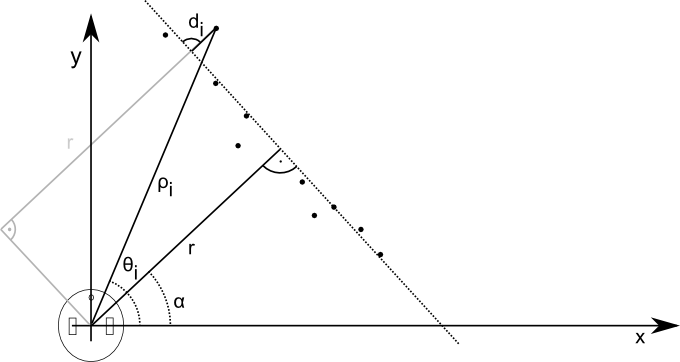
\includegraphics[width=\textwidth]{figs/linefitting.png}
	% \caption{A 2D point cloud recorded by a laser-scanner or similar device. A line (dashed) is fitted through the points in a least-square sense.}
	\caption{由激光扫描仪或类似设备记录的2D点云。线(虚线)以最小二乘的方式穿过点。}
	\label{fig:linefitting}
\end{figure}

% \subsection{Line fitting using least squares}
\subsection{使用最小二乘法的线拟合}
% Using simple trigonometry we can now write

使用简单的三角学我们现在可以写为

\begin{equation}
\rho_i \cos(\theta_i-\alpha)-r=d_i.
\end{equation}

% Different line candidates --- parametrized by $ r$ and $ \alpha$ --- will have different values for $ d_i$. We can now write an expression for the total error $ S_{r,\alpha}$ as

由$r$和$\alpha$---进行参数化的不同行候选人对于$d_i$将具有不同的值。现在我们可以为总错误$S_{r,\alpha}$写一个表达式


\begin{equation}
S_{r,\alpha}=\sum_{i=1}^{N}{d_i^2}=\sum_i(\rho_i \cos(\theta_i-\alpha)-r)^2
\end{equation}

% Here, we square each individual error to account for the fact that a negative error, i.e.\a po int left of the line, is as bad as a positive error, i.e.\a po int right of the optimal line. In order to optimize $ S_{r,\alpha}$, we need to take the partial derivatives with respect to $ r$ and $ \alpha$, set them zero, and solve the resulting system of equations for $ r$ and $ \alpha$.

在这里,我们将每个单独的错误换算成一个事实,即负的错误,即,该行左边的一个点与正误差一样差,即最佳行的点右边。为了优化$S_{r,\alpha}$,我们需要对$r$和$\alpha$采用偏导数,将它们设置为零,然后解决生成的$r$和$\alpha$的方程组。


\begin{equation}
\frac{\partial{S}}{\partial{\alpha}}=0 \qquad \frac{\partial{S}}{\partial{r}}=0
\end{equation}

% Here, the symbol $ \partial$ indicates that we are taking a partial derivative. Solving for $r$ and $\alpha$ is involved, but possible \cite{siegwart2011introduction}:

这里,符号$\partial$表示我们正在进行偏导数。解决$r$和$\alpha$涉及,但可能\cite{siegwart2011introduction}:

\begin{equation}\label{eq:linealpha}
\alpha=\frac{1}{2}atan\left(\frac{\frac{1}{N}\sum{\rho_i^2 sin 2\theta_i}-\frac{2}{N^2}\sum{\sum{\rho_i\rho_j cos \theta_i sin \theta_j}}}{\frac{1}{N}\sum{\rho_i^2 cos 2 \theta_i - \frac{1}{N^2}\sum{\sum{\rho_i \rho_j cos(\theta_i+\theta_j)}}}}\right)
\end{equation}

and
\begin{equation}\label{eq:liner}
r=\frac{{\sum \rho_i cos (\theta_i-\alpha)}}{N}
\end{equation}

% We can therefore calculate the distance and orientation of a wall captured by our proximity sensors relative to the robot's positions or the height and orientation of a line in an image based on a collection of points that we believe might belong to a line.

% This approach is known as the \emph{least-square method}\index{Least-Square Method (Line fitting)} and can be used to fit data to any parametric model. The general approach is to describe the fit between the data and the model in terms of an error. The best fit will minimize this function, which will therefore have a zero derivative at this point. If the result cannot be obtained analytically as in this example, numerical methods have to be used to find the best fit that minimizes the quadratic error.


因此,我们可以基于我们认为可能属于一条线的点的集合来计算由接近传感器相对于机器人的位置或图像中的线的高度和方向捕获的壁的距离和方向。

这种方法称为\emph{最小二乘法}\index{最小二乘法(线拟合)},可用于将数据拟合到任何参数模型中。一般的方法是根据错误来描述数据和模型之间的拟合。最佳拟合将最小化这个功能,因此在这一点上将会有一个零导数。如果在本例中不能得到分析结果,则必须使用数值方法来找出最小化二次误差的最佳拟合。


% \subsection{Split-and-merge algorithm}
% A key problem with this approach is that it is often unclear how many lines there are and where a line starts and where it ends. Looking through the camera, for example, we will see vertical lines corresponding to wall corners and horizontal ones that correspond to wall-floor intersections and the horizon; using a distance sensor, the robot might detect a corner. We therefore need an algorithm that can separate point clouds into multiple lines. One possible approach is to find the outlier with the strongest deviation from a fitted line and split the line at this point. This is illustrated in Figure \ref{fig:splitandmerge}. This can be done iteratively until each line has no outliers above a certain threshold. 

\subsection{分割和合并算法}
这种方法的一个关键问题是,通常不清楚有多少行,以及一行开始以及结束的位置。例如,通过相机,我们将看到对应于墙壁交叉点和地平线的墙角和水平线的垂直线;使用距离传感器,机器人可能会检测到一个角落。因此,我们需要一种可将点云分成多行的算法。一种可能的方法是找出具有与拟合线最强偏离的异常值,并在此点分割线。这在图\ref{fig:splitandmerge}中说明。这可以迭代地进行,直到每一行都没有高于某个阈值的异常值。


\begin{figure}
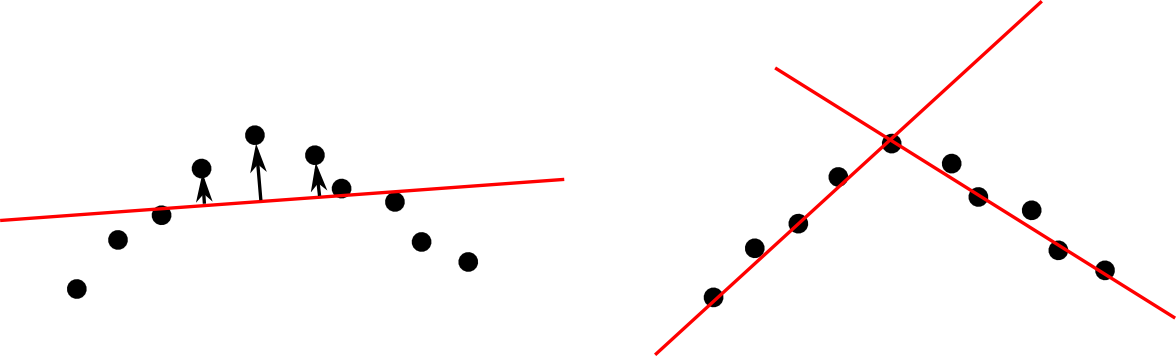
\includegraphics[width=\textwidth]{figs/splitandmerge}
% \caption{Split-and-merge algorithm. Initial least-square fit of a line (left). Splitting the data-set at the point with the highest error (after picking a direction) allows fitting two lines with overall lesser error.\label{fig:splitandmerge}} 
\caption{
分割和合并算法。线的初始最小二乘拟合(左)。在具有最高误差的点上分割数据集(在选择方向之后)允许拟合两条总体较小误差的线。
\label{fig:splitandmerge}} 
\end{figure}

% \subsection{RANSAC: Random Sample and Consensus}
% If the number of ``outliers'' are large, a least square fit will generate poor results as it will generate the ``best'' fit that accomodates both ``inliers'' and ``outliers''. Also, split-and-merge algorithms will fail as they are extremely susceptive to noise: depending on the actual parameters every outlier will split a potential line into two. A solution to this problem is to randomly sample possible lines and keep those that satisfy a certain desired quality given by the number of points being somewhat close to the best fit. This is illustrated in Figure \ref{fig:ransac}, with darker lines corresponding to better fits. RANSAC\index{RANSAC}\index{Random Sample and Consensus} usually requires two parameters, namely the number of points required to consider a line to be a valid fit, and the maximum $d_i$ from a line to consider a point an inlier and not an outlier. The algorithm proceeds as follows: select two random points from the set and connect them with a line. Grow this line by $d_i$ in both directions and count the number of inliers. Repeat this until one or more lines that have sufficient number of inliers are found, or a maximum number of iterations are reached.

\subsection{RANSAC:Random Sample and Consensus}
如果“异常值”的数量很大,则最小二乘拟合将产生不良结果,因为它会产生适应“内部”和“异常值”的“最佳”匹配。此外,拆分和合并算法将会失败,因为它们对噪声非常敏感:根据实际参数,每个异常值都将可能的线分成两部分。这个问题的解决方案是随机抽取可能的线,并保持那些满足一定的期望质量的点数,这些点数靠近最佳拟合点。这在图\ref{fig:ransac}中示出,其中较暗的线对应于更好的拟合。RANSAC\index{RANSAC}\index{Random Sample and Consensus}通常需要两个参数,即将行视为有效拟合所需的点数,以及一行中最大$d_i$来考虑一个入口点而不是异常值。算法进行如下:从集合中选择两个随机点,并将其与一行连接。在两个方向上增加$d_i$这一行,并计算内部值的数量。重复此操作,直到找到具有足够数量的内部值的一行或多行,或者达到最大次数。


\begin{figure}
\center
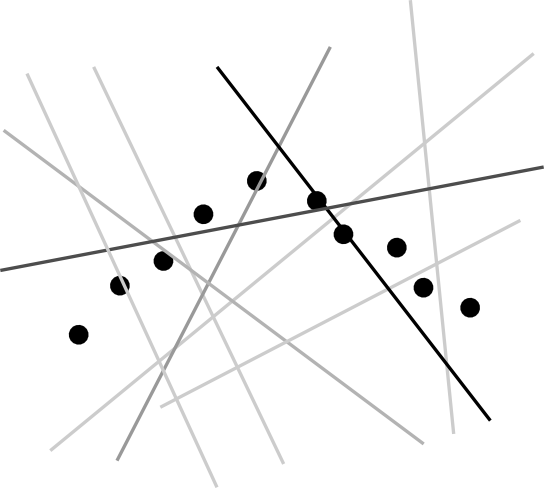
\includegraphics[width=0.6\textwidth]{figs/ransac}
% \caption{Random Sample and Consensus (RANSAC). Random lines are evaluated by counting the number of points close by (''inliers''), darker lines are better fits.\label{fig:ransac}} 
\caption{
随机抽样与共识(RANSAC)。随机行通过计数靠近(“内在”)的点数来评估,较暗的行更适合。
\label{fig:ransac}} 
\end{figure}

% The RANSAC algorithm is fairly easy to understand in the line fitting application, but can be used to fit arbitrary parametric models to any-dimensional data. Here, its main strength is to cope with noisy data.

% Given that RANSAC is random, finding a really good fit will take quite some time. Therefore, RANSAC is usually used only as a first step to get an initial estimate, which can then be improved by some kind of local optimization, such as least-squares, e.g.

RANSAC算法在线拟合应用中相当容易理解,但可用于将任意参数模型拟合为任意维数据。 在这里,它的主要优点是应对嘈杂的数据。

鉴于RANSAC是随机的,找到一个非常好的合适将需要相当长的一段时间。因此,RANSAC通常仅用作获得初始估计的第一步骤,然后可以通过某种局部优化来改进,例如最小二乘法,例如最小二乘法。


% \subsection{The Hough Transform}
% The Hough transform \index{Hough transform} can best be understood as a voting scheme to guess the parametrization of a feature such as a line, circle or other curve \cite{duda1972use}. For example, a line might be represented by $y=mx+c$, where $m$ and $c$ are the gradient and offset. A point in this parameter space (or ``Hough-space'') then corresponds to a specific line in $x-y$-space (or ``image-space''). The Hough-transform now proceeds as follows: for every pixel in the image that could be part of a line, e.g., white pixels in a thresholded image after Sobel filtering, construct all possible lines that intersect this point. (Drawing an image of this would look like a star). Each of these lines has a specifc $m$ and $c$ associated with it, for which we can add a white dot in Hough-space. Continuing to do this for every pixel of a line in an image will yield many $m-c$ pair, but only one that is common among all those pixels of the line in the image: the actual $m-c$ parameters of this line. Thinking about the number of times a point was highlighted in Hough-space as brightness, will turn a line in image space into a bright spot in Hough-space (and the other way round). In practice, a polar representation is chosen for lines. This is shown in Figure \ref{fig:hough}. The Hough transform also generalizes to other parametrization such as circles.  

\subsection{霍夫变形}
霍夫变换\index{霍夫变换}最好被理解为一个投票方案来猜测诸如线,圆或其他曲线的特征参数化\cite{duda1972use}。例如,一行可以由$y=mx+c$表示,其中$m$和$c$是渐变和偏移量。此参数空间(或“Hough-space”)中的一个点对应于$x-y$-space(或“image-space”)中的特定行。霍夫变换现在进行如下:对于可能是线的一部分的图像中的每个像素,例如Sobel滤波之后的阈值图像中的白色像素,构造与该点相交的所有可能的线。(绘制一个这样的图像看起来像一颗星星)。这些行中的每一行都有一个特定的$m$和$c$与之相关联,我们可以在Hough空间中添加一个白点。继续为图像中的一行的每个像素执行此操作将产生许多$m-c$对,但只有一个在图像行中的所有像素中是常见的:该行的实际$m-c$参数。想想在霍夫空间突出点亮度的次数,会将图像空间中的一条线变成霍夫空间的亮点(另一方面)。在实践中,线选择极性表示。这显示在图\ref{fig:hough}中。霍夫变换也泛化为其他参数化,如圆形。


\begin{figure}
\center
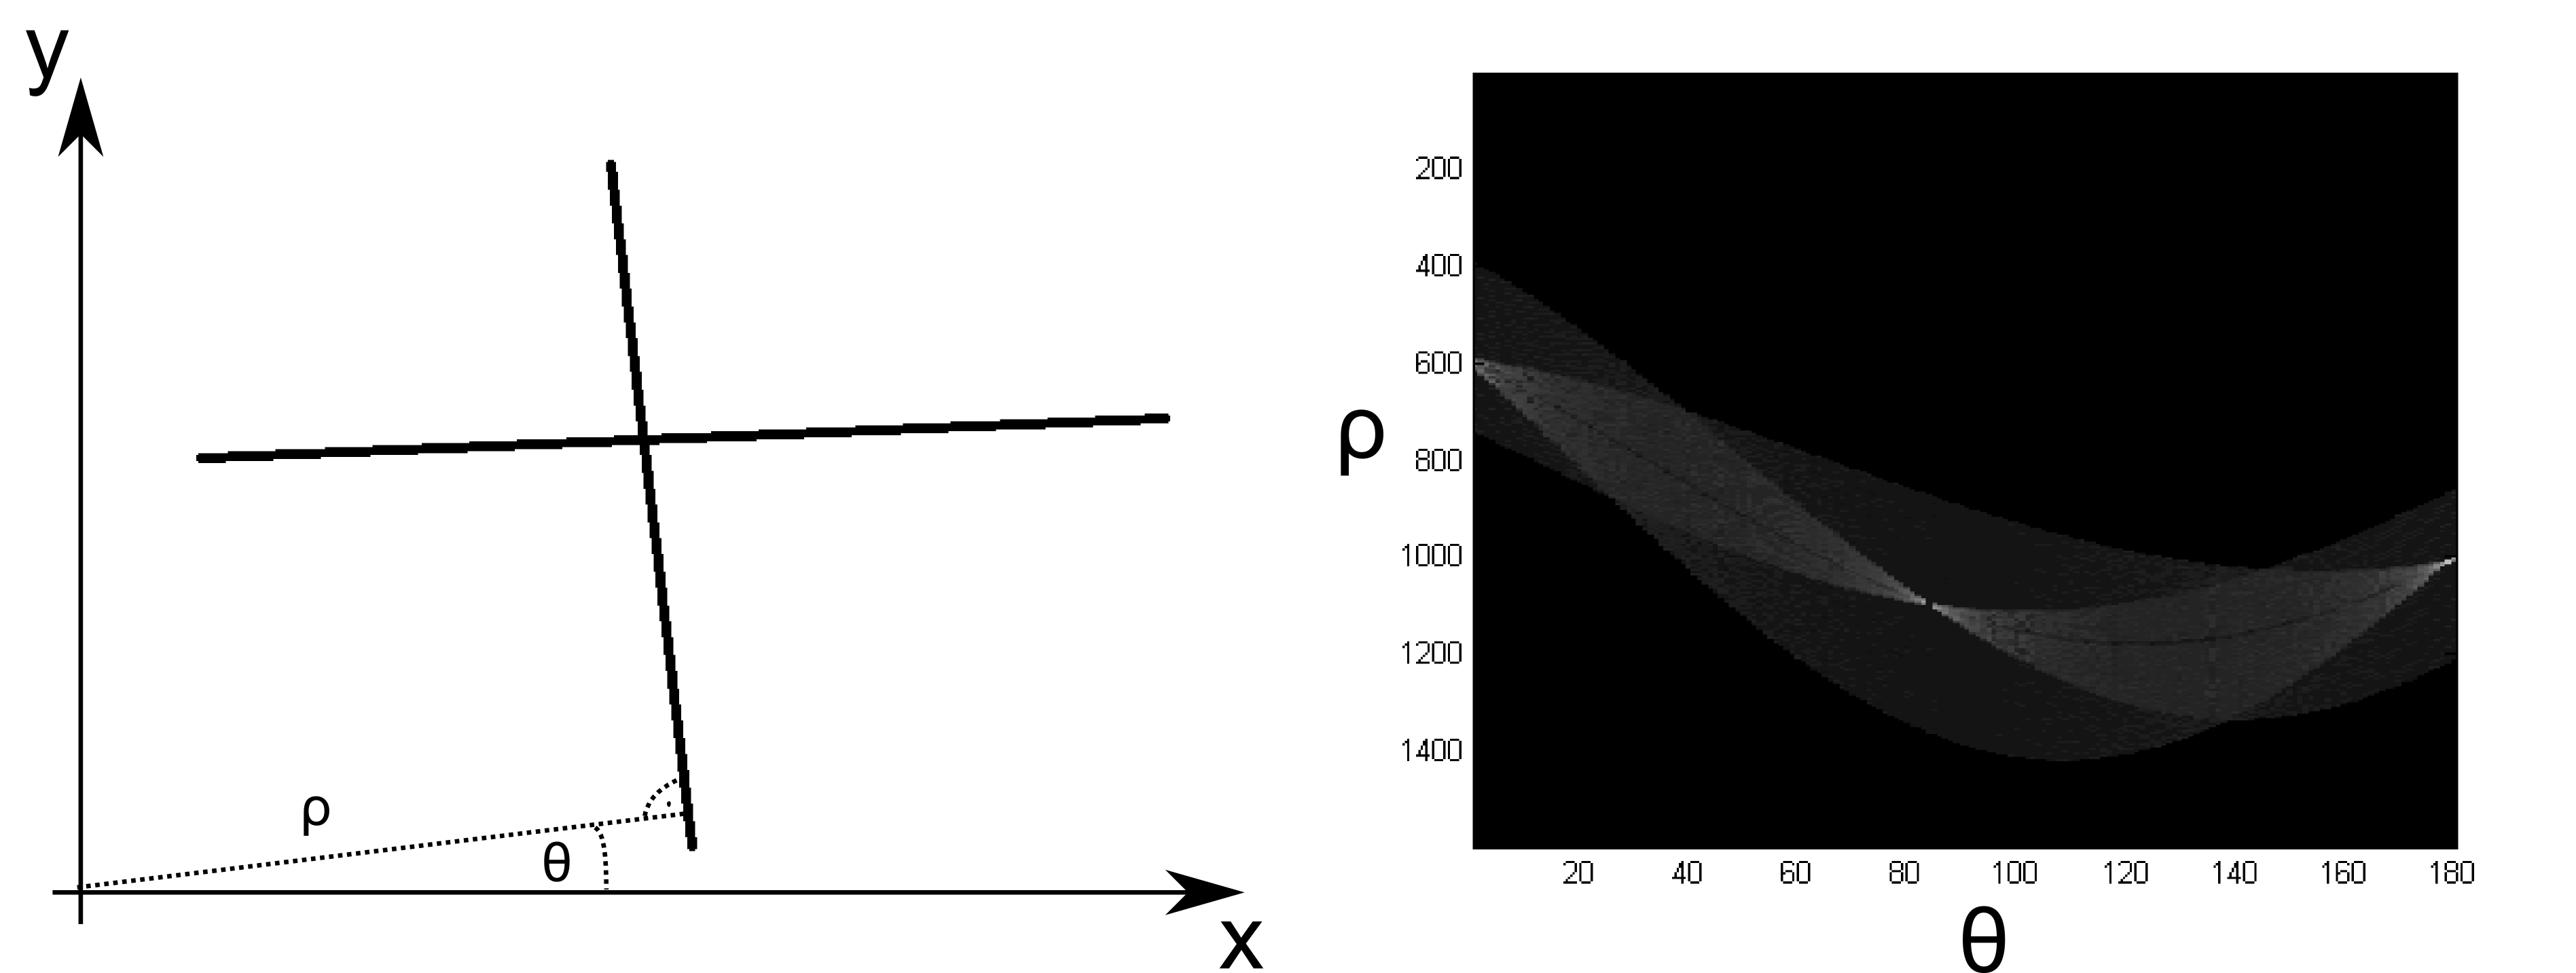
\includegraphics[width=\textwidth]{figs/houghtransform}
% \caption{Lines in an image (left) transposed into Hough-space $\rho$ (distance from origin) and $\theta$ (angle of normal with respect to origin). Bright spots in the Hough image (right) correspond to parameters that have received the most ``votes'' and clearly show the two lines at around 90$^o$ and 180$^o$.\label{fig:hough}} 
\caption{
图像中的线(左)转换为霍夫空间$\rho$(距原点的距离)和$\theta$(相对于原点的正常角度)。霍夫图像中的亮点(右)对应于已经获得最多“投票”的参数,并且清楚地显示了大约$90^o$和$180^o$的两行。
\label{fig:hough}} 
\end{figure}


% \section{Scale-Invariant Feature Transforms}
% Scale-invariant feature transforms are a class of algorithms/signal-processing techniques that allow to extract features that are easily detectable across different scales (or distances to an object), independent of their rotation, and to some extent robust to affine transformations, i.e., views of the same object from different perspectives, and illumination changes. The most prominent in this class is the SIFT algorithm \cite{lowe1999object},\index{SIFT} which however has lost popularity due to closed-source and licensing cost, and has been replaced in the past with SURF (Speed-Up Robust Feature)\index{SURF} and many others,  which are freely available and have slightly different performance and varying use cases. As the math behind SURF is more involved, we focus on the intuition behind SIFT and encourage the reader to download and play with the various open-source implementations of other feature detectors that are available open source.

\section{尺度不变特征变换}
尺度不变特征变换是一类算法/信号处理技术,其允许提取在不同尺度(或距物体的距离)下容易检测的特征,而不依赖于其旋转,并且在某种程度上鲁棒地进行仿射变换,即,从不同角度看待同一个对象,以及照明变化。该类中最突出的是SIFT算法\cite{lowe1999object},\index{SIFT},然而由于封闭源代码和许可成本,该算法已经失去了人气,并且已经被SURF(加速鲁棒特征))\index{SURF}等等,这些都是免费提供的,具有稍微不同的性能和不同的用例。由于SURF背后的数学更多地涉及,我们专注于SIFT背后的直觉,并鼓励读者下载并使用可用的开源的其他特征检测器的各种开放源代码实现。


% \subsection{Overview}
% SIFT proceeds in multiple steps. Descriptions of the algorithm often include its application to object recognition, but these algorithms are independent of feature generation (see below).

\subsection{概述}
SIFT进行多个步骤。该算法的描述通常包括其应用于对象识别,但这些算法与特征生成无关(见下文)。

\begin{enumerate}
% \item Differences of Gaussians (DoG) at different scales:
\item 不同尺度的高斯差异(DoG):

\begin{itemize}
% \item Generate multiple scaled versions of the same image by re-sampling every 2nd, 4th and so on pixel.
% \item Filtering each scaled picture with various Gaussian filters of different variance.
% \item Calculating the difference between pairs of filtered images. This is equivalent to a DoG filter.

\item 通过对每2,4等像素进行重新采样,生成同一图像的多个缩放版本。
\item 使用不同方差的各种高斯滤波器过滤每个缩放图像。
\item 计算过滤图像对之间的差异。 这相当于DoG过滤器。
\end{itemize}

% \item Detecting local minima and maxima in the DoG images across different scales (Figure \ref{fig:siftrejection}, left) and reject those with low contrast (Figure \ref{fig:siftrejection}, right). 

\item 检测不同尺度的DoG图像中的局部最小值和最大值(图\ref{fig:siftrejection},左),并拒绝那些具有低对比度的图像(图\ref{fig:siftrejection},右)。

\begin{figure}
	\centering
		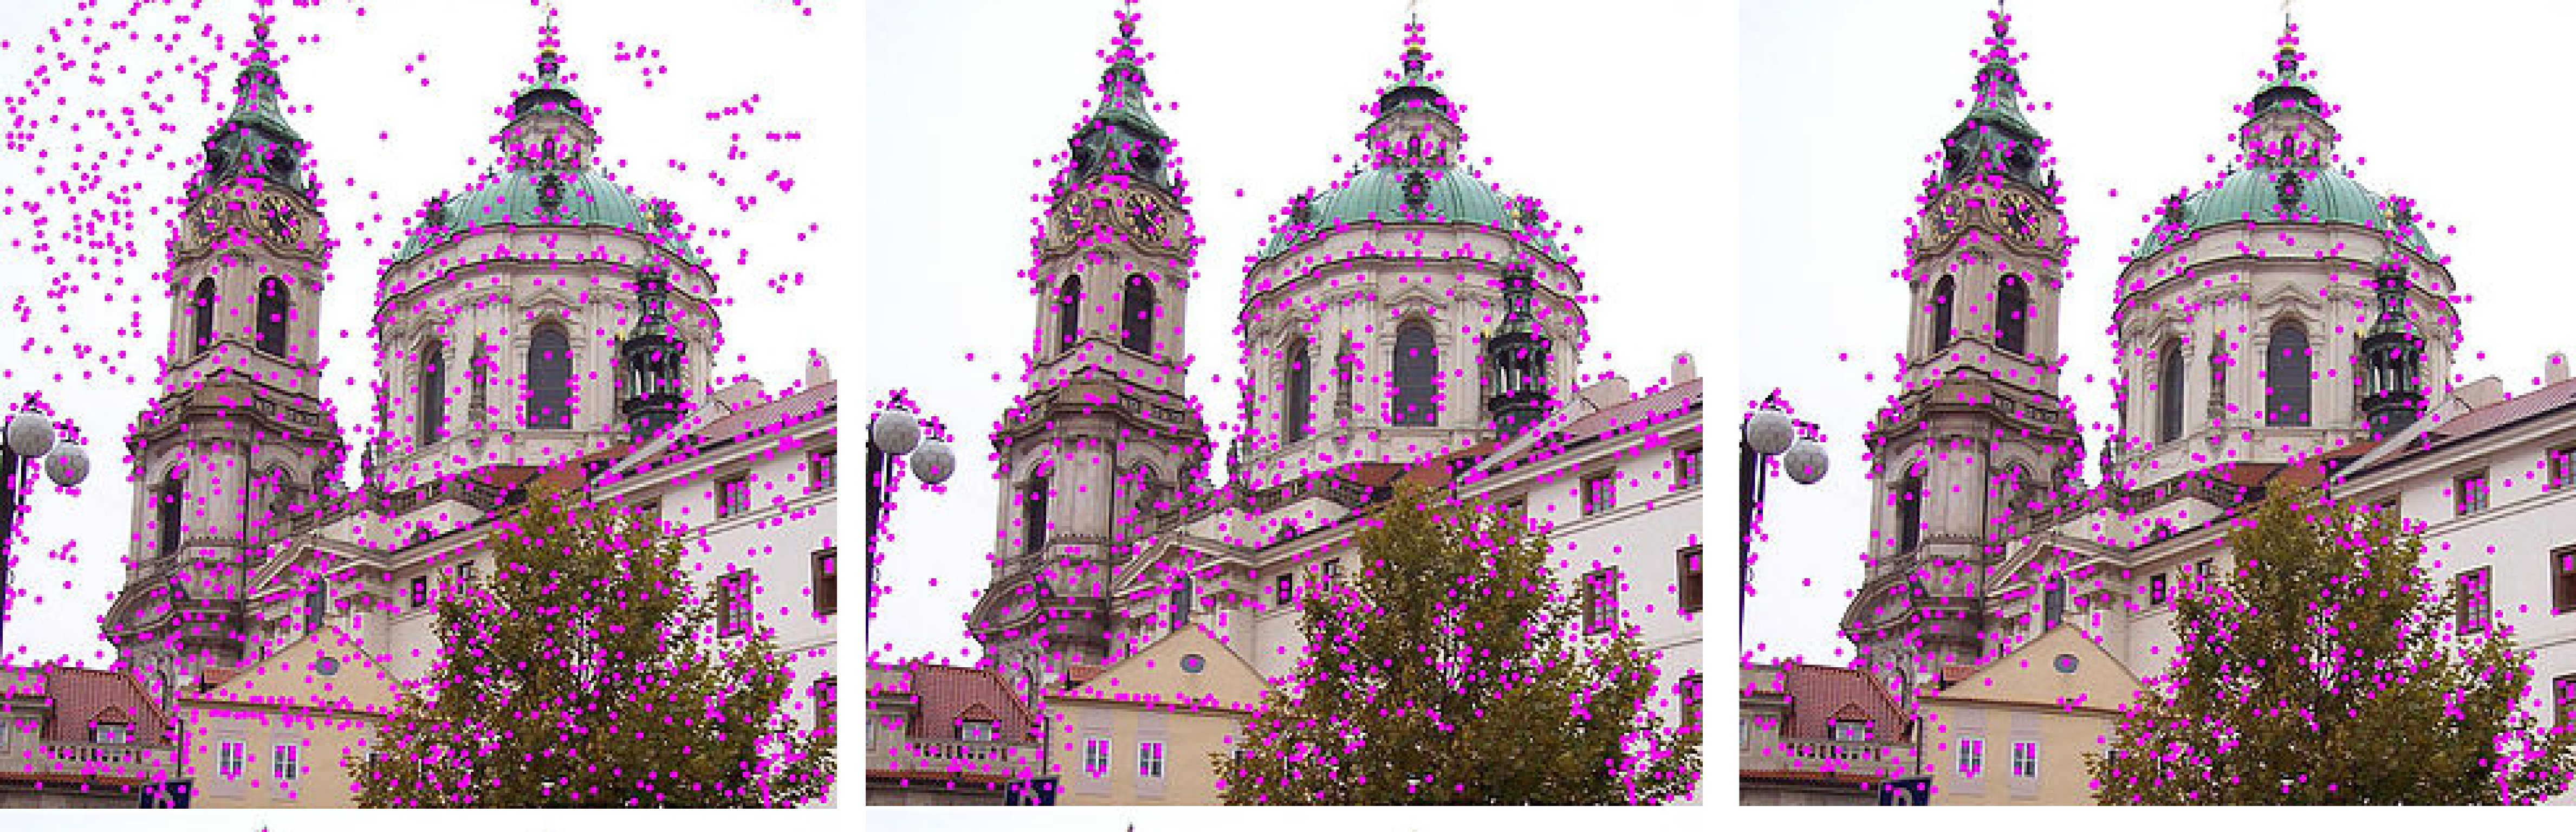
\includegraphics[width=\textwidth]{figs/siftrejection.png}
	% \caption{After scale space extrema are detected (left), the SIFT algorithm discards low contrast keypoints (center) and then filters out those located on edges (right). \copyright Lukas Mach CC-BY 3.0}
	\caption{在检测到尺度空间极值(左)后,SIFT算法丢弃低对比度关键点(中心),然后过滤掉位于边缘(右)的那些。 \copyright Lukas Mach CC-BY 3.0}
	\label{fig:siftrejection}
\end{figure}

% \item Reject extrema that are along edges by looking at the second derivative around each extrema (Figure \ref{fig:siftrejection}, right). Edges have a much larger principal curvature across them than along them.
% \item Assign a ``magnitude'' and ``orientation'' to each remaining extrema (keypoint). The magnitude is the squared difference between neighboring pixels and the orientation is the angle between magnitude along the y-axis vs. magnitude along the x-axis. These calculations are made for all pixels in a fixed neighborhood around the initial keypoint, e.g., in a 16x16 pixel neighborhood.
% \item Collect orientations of neighboring pixels in a histogram, e.g., 36 bins each covering 10 degrees. Maintain the orientation corresponding to the strongest peak and associate it with the keypoint.
% \item Repeat step 4, but for four 4x4 pixel areas around the keypoint in the image scale that has the most extreme minima/maxima. Here, only 8 bins are used for the orientation histogram. As there are 16 histograms in a 16x16 pixel area, the feature descriptor has 128 dimensions.
% \item The feature descriptor vector is normalized, tresholded, and again normalized to make it more robust against illumination changes.
% \item Local gradient magnitude and orientation are grouped into bins and create a 128-dimensional feature descriptor.

\item 通过查看每个极值周围的二阶导数来拒绝边缘的极值(图\ref{fig:siftrejection},右)。边缘上的主曲率比沿着它们大得多。
\item 为每个剩余的极值(关键点)分配一个“大小”和“方向”。大小是相邻像素之间的平方差,取向是沿着y轴的幅度与沿x轴的幅度之间的角度。这些计算是针对初始关键点周围的固定邻域中的所有像素进行的,例如在16×16像素邻域中。
\item 收集直方图中相邻像素的方向,例如每个覆盖10度的36个仓。保持与最强峰对应的方向,并将其与关键点相关联。
\item 重复步骤4,但对于具有最极端最小值/最大值的图像尺度中的关键点周围的四个4x4像素区域。在这里,方向直方图只使用8个空格。由于16x16像素区域中有16个直方图,所以特征描述符具有128个维度。
\item 特征描述符向量被归一化,阈值化,并再次归一化,使其对照明变化更加鲁棒。
\item 局部梯度大小和方向被分组成仓并创建128维特征描述符。

\end{enumerate}

% The resulting 128 dimensional feature vectors are now scale-invariant (due to step 2), rotation-invariant (due to step 5), and robust to illumination changes (due to step 7).

所得到的128维特征向量现在是按比例不变的(由于步骤2),旋转不变量(由于步骤5)),并且对照明变化(由于步骤7)是鲁棒的。

% \subsection{Object Recognition using scale-invariant features}
% Scale-invariant features of training images can be stored in a database and can be used to identify these objects in the future. This is done by finding all features in an image and comparing them with those in the database. This comparison is done by using the Euclidian distance as metric and searching a k-d tree (with d=128). In order to make this approach robust, each object needs to be identified by at least 3 independent features. For this, each descriptor stores the location, scale and orientation of it relative to some common point on the object. This allows each detected feature to ``vote'' for the position of the object that it is most closely associated with in the database.  This is done using a Hough-transform. For example, position (2 dimensions) and orientation (1 dimension) can be discretized into bins (30 degree width for orientation); bright spots in Hough-space then correspond to an object pose that has been identified by multiple features.

\subsection{使用比例不变特征的对象识别}
训练图像的尺度不变特征可以存储在数据库中,并可用于在将来识别这些对象。这是通过查找图像中的所有功能并将其与数据库中的功能进行比较来完成的。该比较通过使用欧几里得距离作为度量并搜索k-d树(d=128)来完成。为了使这一方法变得稳健,每个对象需要通过至少3个独立的特征来识别。为此,每个描述符存储相对于对象上的某些公共点的位置,比例和方向。这允许每个检测到的特征对于与数据库中最密切相关联的对象的位置进行“投票”。这是使用霍夫变换完成的。例如,位置(2维)和取向(1维)可以离散成箱子(取向为30度宽度);霍夫空间中的亮点然后对应于已被多个特征识别的物体姿势。

% \section*{Take-home lessons}
\section*{课后补充}
\begin{enumerate}
% \item Features are ``interesting'' information in sensor data that are robust to variations in rotation and scale as well as noise.
% \item Which features are most useful depends on the characteristics of the sensor generating the data, the structure of the environment, and the actual application.
% \item There are many feature detectors available some of which operating as simple filters, others relying on machine learning techniques.
% \item Lines are among the most important features in mobile robotics as they are easy to extract from many different sensors and provide strong clues for localization.

\item 特征是传感器数据中的“有趣”信息,对于旋转和刻度以及噪声的变化都是鲁棒的。
\item 哪些功能最有用取决于生成数据的传感器的特性,环境结构和实际应用。
\item 有许多功能检测器可用,其中一些作为简单的过滤器,其他功能检测器依靠机器学习技术。
\item 行是移动机器人中最重要的功能之一,因为它们易于从许多不同的传感器中提取,并为本地化提供强大的线索。
\end{enumerate}

% \section*{Exercises}\small
\section*{习题}\small
\begin{enumerate}
% \item Think about what information would make good features in different operating scenarios: a supermarket, a warehouse, a cave. 
% \item What other features could you detect using a Hough transform? Can you find parameterizations for a circle, a square or a triangle?
% \item Do an online search for SIFT. What other similar feature detectors can you find? Which provide source code that you can use online?
% \item A line can be represented by the function $y=mx+c$. Then, the Hough-space is given by a 2D coordinate system spanned by $m$ and $c$.

\item 想想什么信息会在不同的操作场景下产生好的功能:超市,仓库,洞穴。
\item 您可以使用霍夫变换检测哪些其他功能?你能找到一个圆,一个正方形或三角形的参数化?
\item 在线搜索SIFT。 你能找到什么其他类似的功能检测器? 哪些提供可以在线使用的源代码?
\item 一行可以由函数$ y = mx + c $表示。然后,霍夫空间由一个由$ m $和$ c $所跨越的二维坐标系统给出。
\begin{enumerate}
% \item Think about a line representation in polar coordinates. What components has the Hough-space in this case?
% \item Derive a parameterization for a circle and describe the resulting Hough space.

\item 想想极坐标中的线表示。在这种情况下,什么组件有霍夫空间?
\item 导出圆的参数化,并描述生成的霍夫空间。
\end{enumerate}
\end{enumerate}
\normalsize